%% !TEX TS-program = pdflatex
%% !TEX encoding = UTF-8 Unicode

\documentclass[10pt]{article} % use larger type; default would be 10pt

\usepackage[utf8]{inputenc} % set input encoding (not needed with XeLaTeX)

%%% Examples of Article customizations
% These packages are optional, depending whether you want the features they provide.
% See the LaTeX Companion or other references for full information.

%%% PAGE DIMENSIONS
\usepackage{geometry} % to change the page dimensions
\geometry{a4paper} % or letterpaper (US) or a5paper or....
\usepackage{setspace}
\usepackage{parskip}
\parskip=1\baselineskip %\advance\parskip by 0pt plus 2pt% to change between paragraphs space
% \geometry{margin=2in} % for example, change the margins to 2 inches all round
% \geometry{landscape} % set up the page for landscape
%   read geometry.pdf for detailed page layout information

% \usepackage{gravarphicx} % support the \includegravarphics command and options

% \usepackage[parfill]{parskip} % Activate to begin paragraphs with an empty line rather than an indent

%%% PACKAGES
\usepackage{booktabs} % for much better looking tables
\usepackage{array} % for better arrays (eg matrices) in maths
\usepackage{paralist} % very flexible & customisable lists (eg. enumerate/itemize, etc.)
\usepackage{verbatim} % adds environment for commenting out blocks of text & for better verbatim
\usepackage{subfig} % make it possible to include more than one captioned figure/table in a single float
% These packages are all incorporated in the memoir class to one degree or another...
\usepackage[fleqn]{amsmath}
\usepackage{amssymb}
\usepackage{enumitem}
\usepackage{amsthm}
\newtheorem{definition}{Definition}
\usepackage{graphicx}
% \graphicspath{ {../Replication/Shimer_2005/XING_Rep_mFile} }
\usepackage{filecontents}
\usepackage{natbib}
\usepackage{scrextend}
\usepackage[table,xcdraw]{xcolor}
\usepackage{tabularx}
\usepackage{multirow}
\usepackage{lscape}
\usepackage{longtable}
\usepackage{booktabs}
% \usepackage{subcaption}
\usepackage{caption}





%%% HEADERS & FOOTERS
\usepackage{fancyhdr} % This should be set AFTER setting up the page geometry
\pagestyle{fancy} % options: empty , plain , fancy
\renewcommand{\headrulewidth}{0pt} % customise the layout...
\lhead{}\chead{}\rhead{}
\lfoot{}\cfoot{\thepage}\rfoot{}

%%% SECTION TITLE APPEARANCE
\usepackage{sectsty}
\allsectionsfont{\rmfamily\bfseries\upshape} % (See the fntguide.pdf for font help)
% (This matches ConTeXt defaults)

%%% ToC (table of contents) APPEARANCE
\usepackage[nottoc,notlof,notlot]{tocbibind} % Put the bibliography in the ToC
\usepackage[titles,subfigure]{tocloft} % Alter the style of the Table of Contents
\renewcommand{\cftsecfont}{\rmfamily\mdseries\upshape}
\renewcommand{\cftsecpagefont}{\rmfamily\mdseries\upshape} % No bold!

\usepackage[colorlinks,citecolor=black,urlcolor=black,bookmarks=false,hypertexnames=true]{hyperref} 
%%% END Article customizations
%%% The "real" document content comes below...

\title{ECON6096 Final Report\\
\cite{Shimer2005}}
\author{Xing Mingjie 3036029301}
\date{\today} % Activate to display a given date or no date (if empty),
         % otherwise the current date is printed 

\begin{document}
\maketitle
\section{Model}
\subsection{Model Setup}
    In the adapted model of \cite{Shimer2005}, workers and firms are matched through a matching function.\newline
    On the unemployed worker side, the arrival rate of jobs is 
    \[f(\theta) = \mu \theta^\eta\]
    On the firm side, the recruiting rate is
    \[q(\theta) = \mu \theta^{\eta-1}\]
    where \(\theta\) is the market tightness, defined as \(\theta = v/u\), where \(v\) is the number of vacancies and \(u\) number of unemployed workers.\newline
    The worker's Bellman equation for unemployment value reads 
    \begin{equation}\label{BellmanUnemploy}
        U_p = z + \delta \{f(\theta_p)\mathbb{E}_p W_{p^\prime} + (1-f(\theta_p))\mathbb{E}_p U_{p^\prime}\}.
    \end{equation}
    Their employment value is given by 
    \begin{equation}\label{BellmanEmploy}
        W_p = w_p + \delta \{(1-s)\mathbb{E}_p W_{p^\prime} + s\mathbb{E}_p U_{p^\prime}\}.
    \end{equation}
    Firm's value from hiring is 
    \begin{equation}\label{BellmanHire}
        J_p = p - w_p + \delta (1-s)\mathbb{E}_p J_{p^\prime}.
    \end{equation}
    Its value for keeping a vacancy is 
    \begin{equation}\label{BellmanVacancy}
        V_p = -c + \delta q(\theta_p)\mathbb{E}_p J_{p^\prime}.
    \end{equation}
    Note that \(V_p  \equiv 0 \) is the free entry condition in the equilibrium.\newline
    Productivity \(p\) is the output of a firm-worker pair, where worker gets \(w\) and firm \(p-w\). Chance that a worker becomes unemployed is \(s\).\newline
    The log of productivity follows AR(1) process 
    \begin{equation}\label{productivityprocess}
        \log(p^\prime) = \rho \log(p) + \varepsilon 
        \end{equation}
        where \[\log(p) \sim N(\mu_{logp}, \sigma^2_{logp}),\ 
        \varepsilon \sim N(\mu_\varepsilon,\sigma^2_\varepsilon)\]
    % In our model setting, \(\mu_\lambda = \mu_\varepsilon = 0, \sigma_\lambda = 0.05, \sigma_\varepsilon = 0.03\).\newline
    The bargaining process between workers and firms is 
    \begin{equation}
        W_p = U_p + \beta (W_p - U_p + J_p)
    \end{equation} which pins down the equilibrium wage \(w\).\newline
    In the equilibrium, workers' inflow equals outflow. So unemployment \(u\) follows
    \[u f(\theta_p) = s(1-u)\]
    
    \subsection{Equilibrium}
    Market tightness \(\theta_p\) is pinned down by solving the following equation of hire rate from free entry condition 
    \begin{equation}\label{HireRate}
    q(\theta_p) = \frac{c}{\delta \mathbb{E}_p J_{p^\prime}}\end{equation}
    Employ Rate is given by \begin{equation}\label{EmployRate}
    f(\theta_p) = \mu^\frac{1}{\eta} q^\frac{\eta-1}{\eta}\end{equation}
    And market tightness \begin{equation}\label{MarketTightness}
    \theta_p = \frac{f(\theta_p)}{q(\theta_p)}\end{equation}
    Optimal wage at each productivity level is given by the Nash Bargaining in the algebra in Appendix \ref{OptWage}: 
    \begin{equation}\label{OptimalWage}
        w_p = \beta p + (1-\beta)z + \beta c \theta_p\end{equation}
    And unemployment rate \begin{equation}\label{UnemployRate}
        u_p = \frac{s}{s + f(\theta_p)}\end{equation}
    
    \begin{definition} \textbf{Equilibrium}
        The definition of equilibrium consists of worker's wage \(w_p\), job arrival rate \(f(\theta_p)\), recruiting rate \(q(\theta_p)\) market tightness \(\theta_p\) and unemployment rate \(u_p\) under productivity level \(p\) which satisfies the process by equation \ref{productivityprocess} such that
            \begin{enumerate}
                \item Recruiting rate satisfies equation \ref{HireRate}.
                \item Job arrival rate satisfies equation \ref{EmployRate}.
                \item Market tightness satisfies equation \ref{MarketTightness}.
                \item The wage of workers satisfies equation \ref{OptimalWage}.
                \item Unemployment rate satisfies equation \ref{UnemployRate}.
            \end{enumerate}

    \end{definition}
\section{Algorithm}
    \subsection{Tauchen method}
    \cite{Tauchen1986} provides a reliable method to simulate the conditional expectations \(\mathbb{E}_p J_{p^\prime}, \\ \mathbb{E}_p U_{p^\prime}, \mathbb{E}_p W_{p^\prime}\) in the value functions. For AR(1) process \ref{productivityprocess}, taking $F$ as representative value function, instead of computing the integral \(\mathbb{E}[F(p^\prime|p)] = \int_{-\infty}^{\infty}F(p^\prime)f(p^\prime|p)dp^\prime\), we can take a finite set \(\Lambda_{logp} = \{logp_1, \ldots, logp_n\}\) and derive a probability transition matrix where \(p_{i,j}=\textbf{Prob} (\tilde{p^\prime} = p_j | \tilde{p} = p_i)\) based on the distribution of stochastic part of the process, so that the conditional expectation can be solved numerically with formula \[\mathbb{E}[F(p^\prime|p)] =\sum\limits_{j=1}^{n}p_{i,j}F(p^\prime).\]
    We know that $logp^\prime$ is normally distributed with mean 0 and standard deviation $\sigma_\varepsilon$, we choose the finite set $\Lambda_{logp}$ to be evenly-spaced along the real line, the upper and lower bound of the set to be \(\mu_{logp} \pm m\sigma_{logp}\) where \(\sigma_{logp} = \sigma_\varepsilon/\sqrt{1-\rho^2}\). Let \(\omega_j = {logp}_j - {logp}_{j-1}\), set the transition matrix to be
    \[p_{i j}= \begin{cases}\Phi\left(\frac{logp_1+\omega_j / 2}{\sigma_{\varepsilon}}\right) & \text { for } j=1 \\ \Phi\left(\frac{logp_j+\omega_j / 2}{\sigma_{\varepsilon}}\right)-\Phi\left(\frac{logp_j-\omega_j / 2}{\sigma_{\varepsilon}}\right) & \text { for } 1<j<n \\ 1-\Phi\left(\frac{logp_n-\omega_j / 2}{\sigma_{\varepsilon}}\right) & \text { for } j=n\end{cases}\] where $\Phi(\cdot)$ is the CDF of normal distribution.
    The grid is set to $p$ with simple transformation $\Lambda_p = \exp{(\Lambda_{logp})}$.
    \newline
    We directly apply \texttt{discretizeAR1\_Tauchen} function from the Matlab Toolbox of \cite{Kirkby2023} to realize the above mentioned Tauchen method.

    \subsection{Discretization}
    The algorithm of discretization method is as follows:
    \begin{enumerate}
        \item Choose a relateive error tolerance level \texttt{tol};
        \item Discretize the state space by constructing a grid for productivity \[
            p = \exp\{logp\}
            \text{\ where\ } logp = \{logp_1, logp_2, \ldots, logp_n\} \] given by the Tauchen method.
            The n is chosen at 5; deviation step is 3. 
        \item Start with an initial guess of the value function \(F^{(0)}(p)\) is a vector of length \(n\), i.e., \(F^{(0)}(p) = \{F^{(0)}_i\}_{i=1}^n\), where \(F^{(0)}_i = F^{(0)}(p_i)\).
            \(F\) here represents \(U, W, J\). The initial guess is \texttt{tol}.
        \label{update}
        \item Update the value function using eqautions \ref{BellmanUnemploy} to \ref{OptimalWage}, specifically
            \begin{enumerate}
                \item Fix the current productivity level at one of the grid points, \(p_i\) from \(i=1\)
                \item For each possible choice of productivity next period, calculate optimal control in the following order:
                \begin{gather*}
                    q(\theta_{p_i}) = \frac{c}{\delta \sum_{j=1}^{n}p_{i,j}J^{(0)}(p_j)}\\
                    f(\theta_{p_i}) = \mu^\frac{1}{\eta} q^\frac{\eta-1}{\eta}\\
                    \theta_{p_i} = f/q\\
                    w_{p_i} = \beta p_i + (1-\beta)z + \beta c \theta_{p_i}
                \end{gather*}
                \item and update the value function system with Jacobi method
                \begin{gather*}
                    U^{(1)}_{p_i} = z + \delta\{f(\theta_{p_i})\sum_{j=1}^{n}p_{i,j}W^{(0)}(p_j) + (1-f(\theta_{p_i}))\sum_{j=1}^{n}p_{i,j}U^{(0)}(p_j)\}\\
                    W^{(1)}_{p_i} = w_{p_i} + \delta\{(1-s)\sum_{j=1}^{n}p_{i,j}W^{(0)}(p_j) + s\sum_{j=1}^{n}p_{i,j}U^{(0)}(p_j)\}\\
                    J^{(1)}_{p_i} = p_i - w_{p_i} + \delta (1-s)\sum_{j=1}^{n}p_{i,j}J^{(0)}(p_j)
                \end{gather*}
                \item Choose a new grid point for productivity, go through 4.1 to 4.3. Once we have done the update for all productivity grid, we have new system of value function \({F^{(1)}_p}\)
                \item Compute distance between the two systems of value functions following the sup L-1 norm \[
                    d = \max\limits_{i\in\{1,\ldots,n\}}|F^{(0)}_i-F^{(1)}_i|\]
                \item If distance is within the error tolerance level, \(d \leq \texttt{tol}\), the functions have converged and go to step 5, or else go back to step 4.
            \end{enumerate}
            \item Calculate the optimal control for each productivity level:
            \begin{gather*}
                q(\theta^*_{p_i}) = \frac{c}{\delta \sum_{j=1}^{n}p_{i,j}J^* (p_j)}\\
                f(\theta^*_{p_i}) = \mu^\frac{1}{\eta} q^\frac{\eta-1}{\eta}\\
                \theta^*_{p_i} = f^* / q^*\\
                w^*_{p_i} = \beta p_i + (1-\beta)z + \beta c \theta^*_{p_i}\\
                u^*_p = \frac{s}{s + f(\theta^*_p)}
            \end{gather*}
            where \(J^*\) is the converged value function.
    \end{enumerate}
    \subsection{Approximation}
    \begin{enumerate}\addtocounter{enumi}{-1}
        \item Since we have discovered that the value function is smooth and monotone, we simply approximate value functions with 4th-order polynomials in accordance with the number of grids \(\hat{F}(p;\textbf{coefs})\) in the form of \[\hat{F}(p; \textbf{coefs}) = a p^4 + bp^3 + cp^2+dp+e \] to match the number of grids. The initial guess of $\textbf{coefs}$ is 70 for $U$ and $W$ and \texttt{tol} for $J$, saved as $\textbf{coefs\_old}$. The stopping criterion is \texttt{tol}. The approximation grid is derived from Tauchen method as done in Discretization.
        \item Calculate the maximized control and value function system with the initial guess with equilibrium condition \ref{HireRate} to \ref{OptimalWage} as
        \begin{gather*}
            q(\theta_{p_i}) = \frac{c}{\delta \sum_{j=1}^{n}p_{i,j}\hat{J}(p_j;\textbf{coefs\_old})}\\
            f(\theta_{p_i}) = \mu^\frac{1}{\eta} q^\frac{\eta-1}{\eta}\\
            \theta_{p_i} = f/q\\
            w_{p_i} = \beta p_i + (1-\beta)z + \beta c \theta_{p_i}
        \end{gather*}
        and Bellman equations \ref{BellmanUnemploy} to \ref{BellmanHire}. 
        \begin{gather*}
            U_{p_i} = z + \delta\{f(\theta_{p_i})\sum_{j=1}^{n}p_{i,j}\hat{W}(p_j;\textbf{W\_coefs\_old}) + (1-f(\theta_{p_i}))\sum_{j=1}^{n}p_{i,j}\hat{U}(p_j;\textbf{U\_coefs\_old})\}\\
            W_{p_i} = w_{p_i} + \delta\{(1-s)\sum_{j=1}^{n}p_{i,j}\hat{W}(p_j;\textbf{W\_coefs\_old}) + s\sum_{j=1}^{n}p_{i,j}\hat{U}(p_j;\textbf{U\_coefs\_old})\}\\
            J_{p_i} = p_i - w_{p_i} + \delta (1-s)\sum_{j=1}^{n}p_{i,j}\hat{J}(p_j;\textbf{J\_coefs\_old})
        \end{gather*}
        Given the smooth property of value functions, we use the Gaussian-Hermite quadrature as in Tauchen's method to calculate the conditional expectation.
        \item Fit for new value function system and report parameters and save as \texttt{new} in an unweighted nonlinear least squares procedure as in \[\min\limits_\textbf{coefs} \sum\limits_{i=1}^{n}(\hat{F}(p_i;\textbf{coefs})-f_i)^2\] and save as \(\textbf{coefs\_new}\) for each value function. $f_i$ stands for the updated value functions $U_{p_i}$, $W_{p_i}$ and $J_{p_i}$ in the maximized procedure. We use Matlab code \texttt{fminsearch} to realize the fitting procedure.
        \item If the largest norm of all value functions statisfies \(||\hat{F}(p;\textbf{coefs\_old})-\hat{F}(p;\textbf{coefs\_new})||<\texttt{tol}\), stop; else go to step 1, replacing \(\textbf{coefs\_old}\) with \(\textbf{coefs\_new}\). We use Matlab code \texttt{norm} to return an Euclidean norm. 
    \end{enumerate}

\section{Quantitative Analysis}
    \subsection{Calibration}
    Parameters calibrated are given in Table \ref{Calibration}. In this first exercise, separation rate $s$ is set to be constant and productivity $p$ a stochastic process with mean 0.
    \begin{table}\centering
        \begin{tabular}{
        >{\columncolor[HTML]{FFFFFF}}l 
        >{\columncolor[HTML]{FFFFFF}}l 
        >{\columncolor[HTML]{FFFFFF}}l }
        \hline\hline
        Parameter         & Symbol                                                & Value \\ \hline
        Productivity std. & $\sigma_{\lambda}$                       & 0.05  \\
        Productivity mean & $\mu_{\lambda}$                          & 0     \\
        Stochastic std.   & $\sigma_{\varepsilon}$ & 0.03  \\
        Stochastic mean   & $\mu_{\varepsilon}$                    & 0     \\
        Separation rate   & $s$                                                     & 0.1   \\
        Discount rate     & $r$                                                     & 0.012 \\
        Value of leisure  & $z$                                                     & 0.4   \\
        Matching function & $\mu$                                                    & 1.355 \\
        Matching function & $\alpha$                                                 & 0.72  \\
        Bargaining Power  & $\beta$                                                  & 0.72  \\
        Cost of vacancy   & $c$                                                     & 0.213 \\ \hline
        \end{tabular}
        \caption{Parameter Calibration}
        \label{Calibration}
        \end{table}

        \subsection{Value function}
        The value function with respect to the productivity level is given by Discretization in Figure \ref{ValueDiscretization} and by Approximation in Figure \ref{ValueApproximation}. Coefficients of each polynomial interpolation of the value functions are reported in Table \ref{coef}, in ascending order of exponent. All value functions growth in monotone with productivity. The employment value is slightly higher than unemployment value, the hiring value slightly higher than vacancy value, which shows that it is always optimal for worker to work and firm hire in equilibrium.

        \begin{figure}
            \centering
            \begin{minipage}{.5\textwidth}
              \centering
              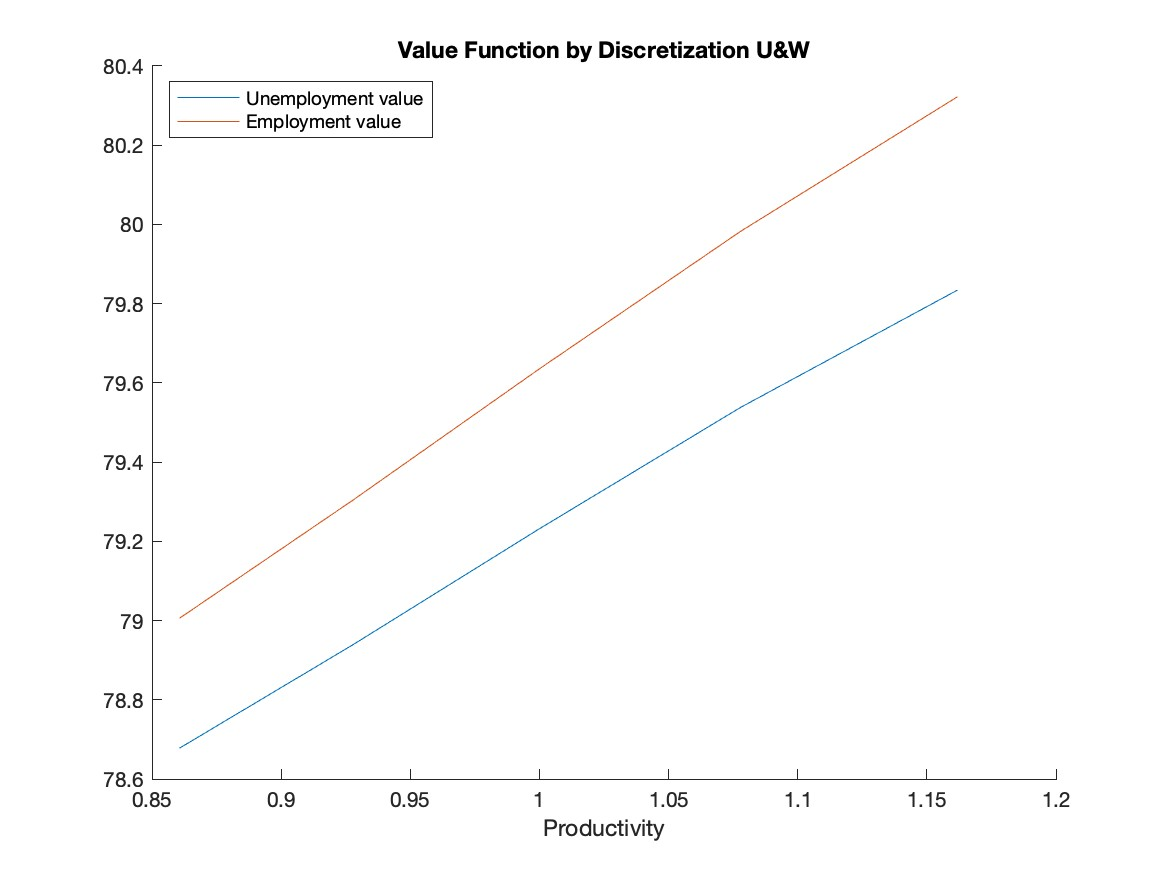
\includegraphics[width=\linewidth]{ValueUWDiscretization}
              \caption{Employ and Unemploy Value}
            \end{minipage}%
            \begin{minipage}{.5\textwidth}
              \centering
              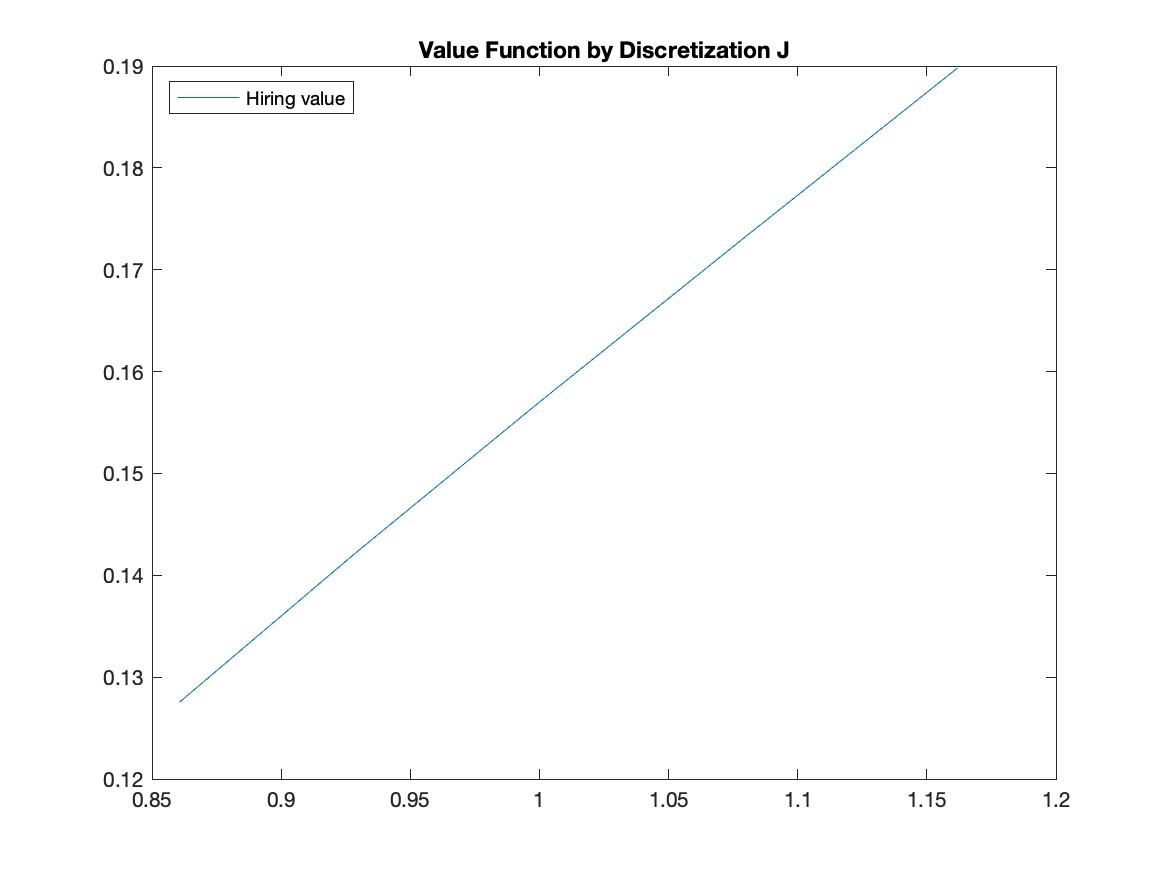
\includegraphics[width=\linewidth]{ValueJDiscretization}
              \caption{Hiring Value}
            \end{minipage}
            \caption{Value Function by Discretization}
            \label{ValueDiscretization}
        \end{figure}

        \begin{figure}
            \centering
            \begin{minipage}{.5\textwidth}
                \centering
                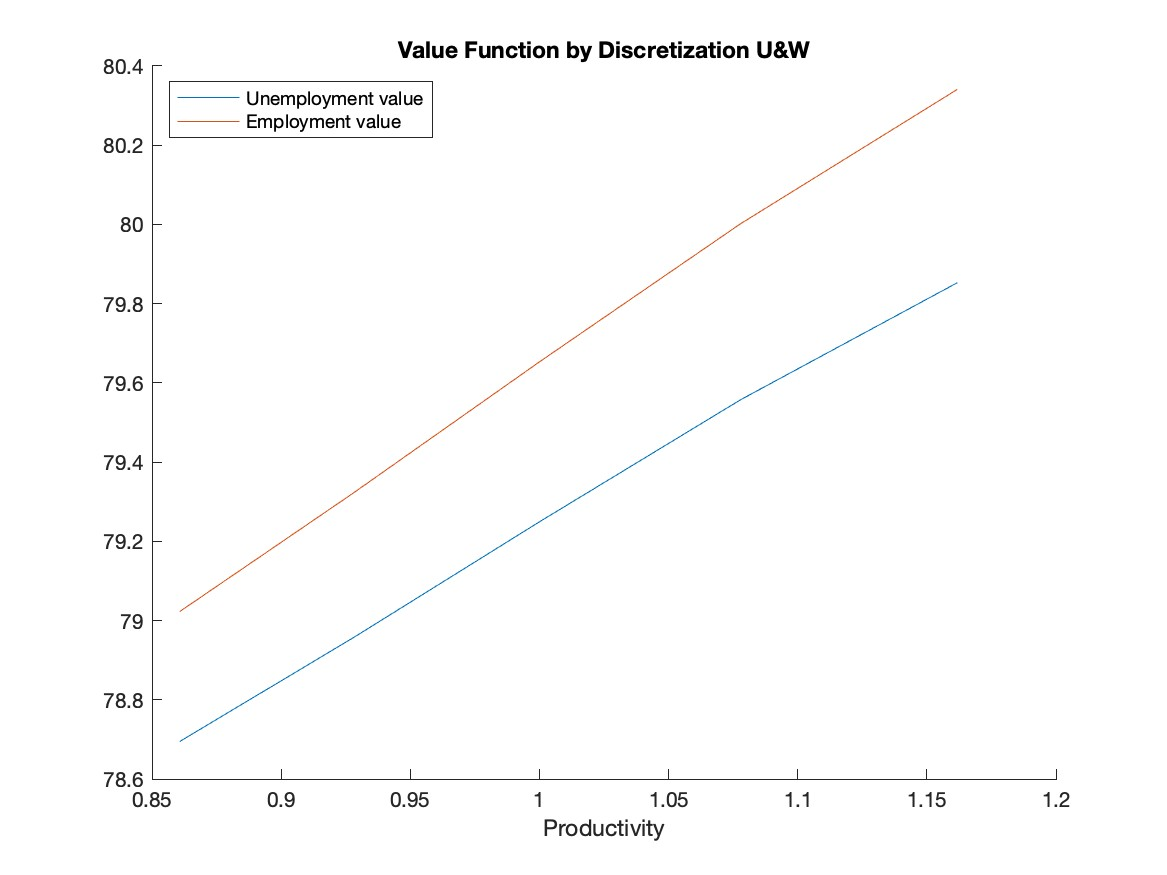
\includegraphics[width=\linewidth]{ValueUWApproximation}
                \caption{Employ and Unemploy Value}
            \end{minipage}%
            \begin{minipage}{.5\textwidth}
                \centering
                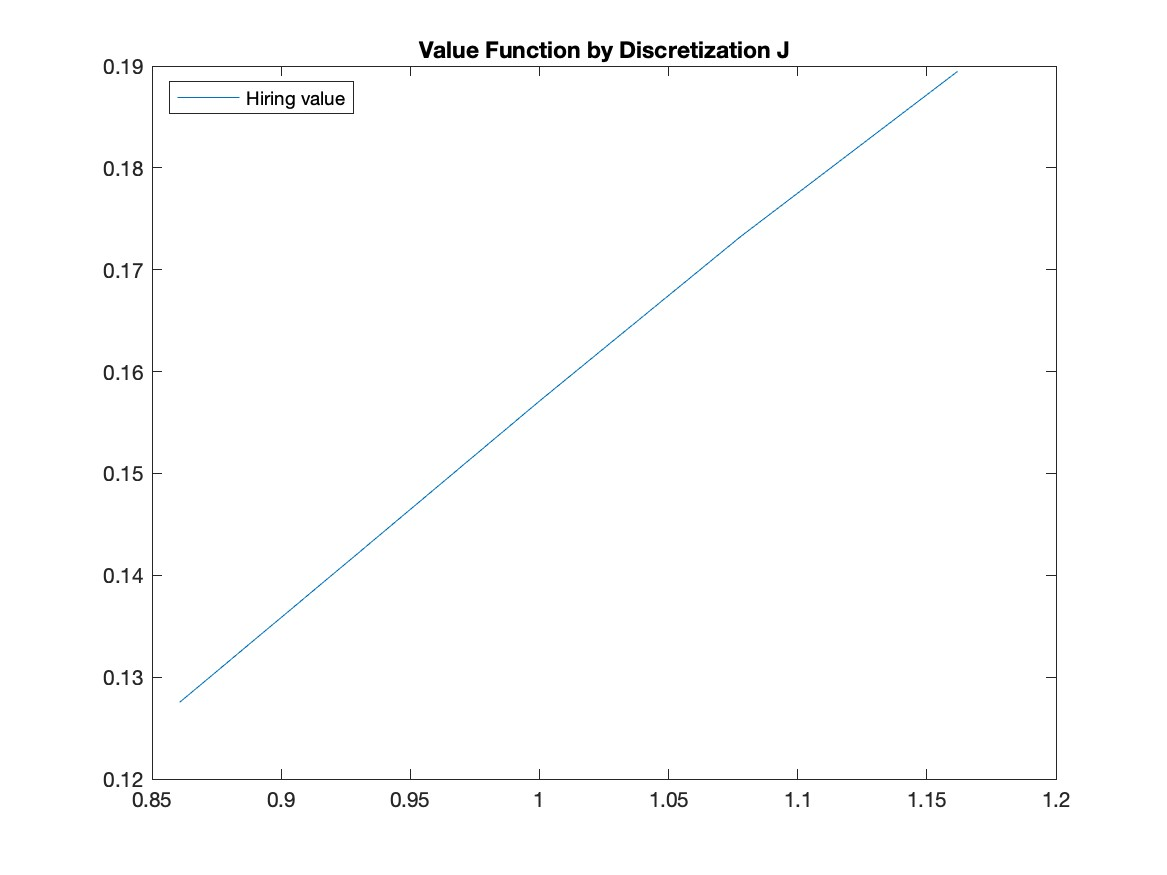
\includegraphics[width=\linewidth]{ValueJApproximation}
                \caption{Hiring Value}
            \end{minipage}
            \caption{Value Function by Approximation}
            \label{ValueApproximation}
        \end{figure}

        \subsection{Control}
        The model fit of control with respect to the productivity level is given by Discretization in Figure \ref{ControlDiscretization} and by Approximation in Figure \ref{ControlApproximation}. The job finding rate and wage grow and unemployment rate falls in monotone to productivity level. Combined with the Value Functions, we can see that a 4-th order Lagrange Interpolation does a good job in approximating the value functions.
        
        \begin{figure}
            \centering
            \begin{minipage}{.5\textwidth}
                \centering
                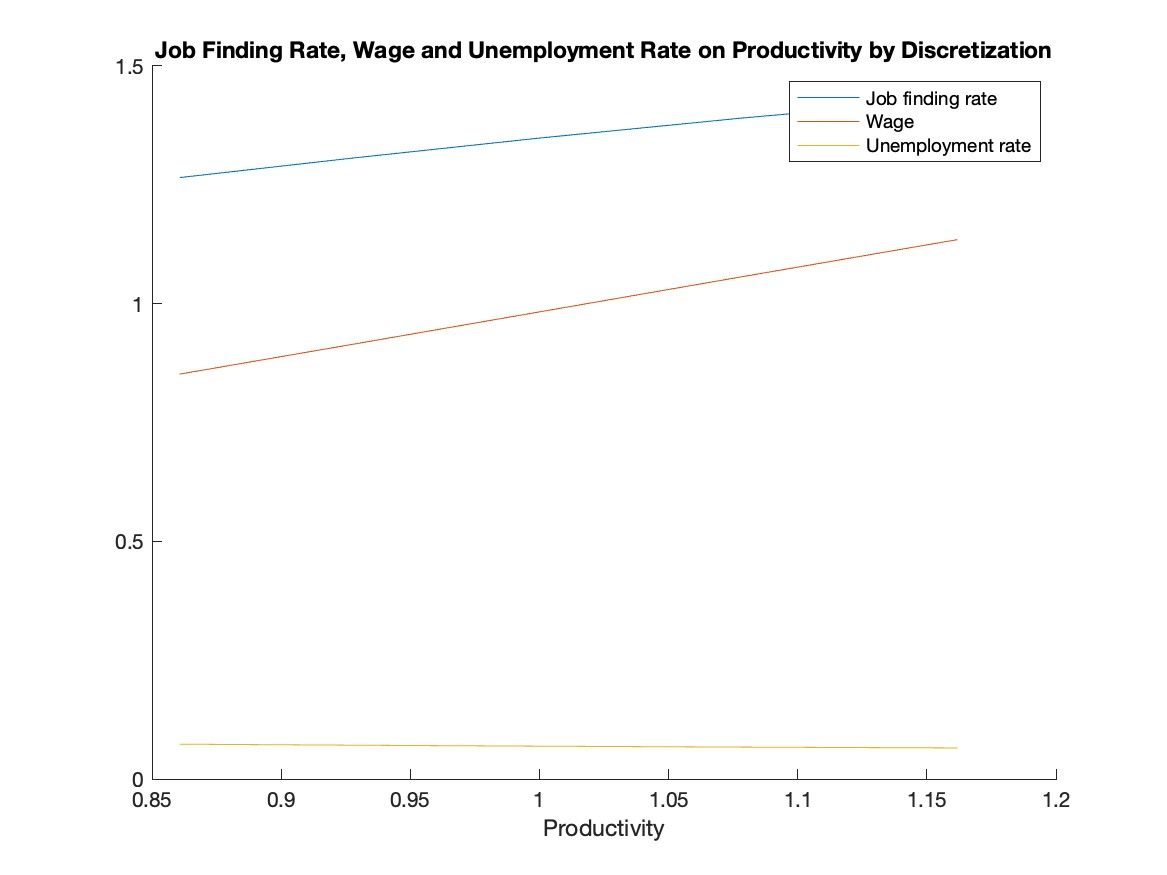
\includegraphics[width=\linewidth]{ControlDiscretization}
                \caption{Control by Discretization}
                \label{ControlDiscretization}
            \end{minipage}%
            \begin{minipage}{.5\textwidth}
                \centering
                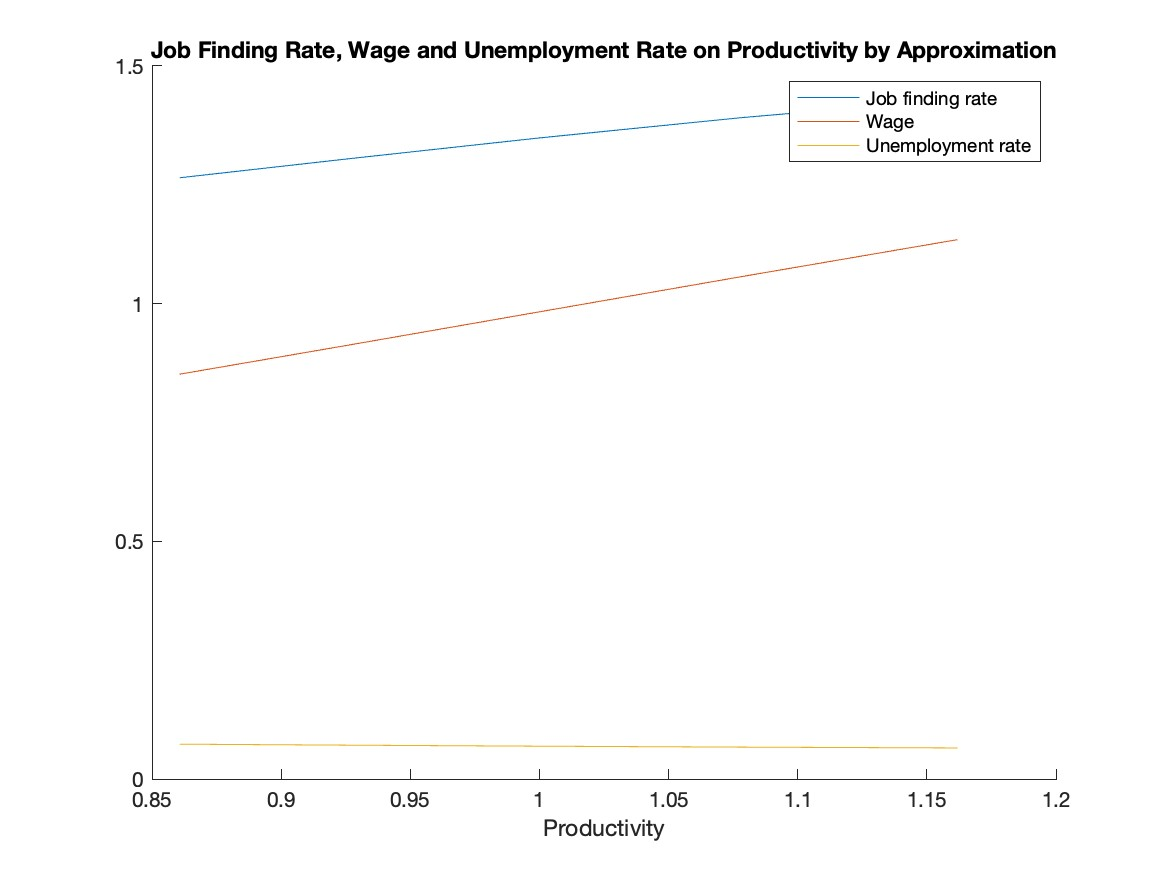
\includegraphics[width=\linewidth]{ControlApproximation}
                \caption{Control by Approximation}
                \label{ControlApproximation}
            \end{minipage}
        \end{figure}

        \begin{table}
            \centering
            \begin{tabular}{
            >{\columncolor[HTML]{FFFFFF}}l 
            >{\columncolor[HTML]{FFFFFF}}c 
            >{\columncolor[HTML]{FFFFFF}}c 
            >{\columncolor[HTML]{FFFFFF}}c }
            \hline\hline
             & \multicolumn{1}{l}{\cellcolor[HTML]{FFFFFF}U} & \multicolumn{1}{l}{\cellcolor[HTML]{FFFFFF}W} & \multicolumn{1}{l}{\cellcolor[HTML]{FFFFFF}J} \\ \hline
            e & 82.567  & 83.090  & -2.42E-04 \\
            d & -18.161 & -20.700 & 0.134     \\
            c & 21.774  & 26.984  & -0.125    \\
            b & -6.395  & -10.203 & 0.267     \\
            a & -0.536  & 0.482   & -0.118    \\ \hline
            \end{tabular}
            \caption{Approximation coefficients}
            \label{coef}
            \end{table}
            
        

        \subsection{Results at typical productivity value}
        The wage, unemployment rate and job finding rate at typical productivity level is given in Table \ref{Qb}
        \begin{table}
            \centering
            \begin{tabular}{
            >{\columncolor[HTML]{FFFFFF}}l 
            >{\columncolor[HTML]{FFFFFF}}l 
            >{\columncolor[HTML]{FFFFFF}}l 
            >{\columncolor[HTML]{FFFFFF}}l }
            \hline\hline
            log(p) & w      & u      & f      \\ \hline
            -0.1  & 0.8930 & 0.0718 & 1.2925 \\
            -0.05 & 0.9367 & 0.0704 & 1.3203 \\
            0     & 0.9827 & 0.0690 & 1.3484 \\
            0.05  & 1.0311 & 0.0677 & 1.3764 \\
            0.1   & 1.0818 & 0.0665 & 1.4039 \\
            \hline
            \end{tabular}
            \caption{Wage, Unemployment rate and Job Finding Rate}
            \label{Qb}
        \end{table}
        

    \subsection{Extended Exercise}
    In this subsection, we calculate the standard deviation of productivity, unemployment rate and job finding rate. The data and model fit standard deviation of productivity, unemployment rate and job finding rate is given in Table \ref{Qc1}. Although the model captures a higher deviation in productivity level, the variation in unemployment and job finding rate is far undermined. \newline
    We also report the correlation matrix of the three variables in Table \ref{corrmain}, correlation between u and f are -0.9994, successfully replicating the empirical result of -0.949, but unemployment correlation with productivity -0.9967, is twice as large as the empirical result (-0.408).  And the job finding rate correlation with productivity is 0.9989, off the target from the data level of 0.396. Correlation between u and v is -0.9980, well capturing the data -0.894. This shows that the baseline model successfully capture the downward slope of the Beveridge curve.
    \begin{table}\centering
        \begin{tabular}{
        >{\columncolor[HTML]{FFFFFF}}l 
        >{\columncolor[HTML]{FFFFFF}}l 
        >{\columncolor[HTML]{FFFFFF}}l 
        >{\columncolor[HTML]{FFFFFF}}l }
        \hline\hline
                  & u   & f     & p     \\ \hline
        Data Std. & 1.90E-01 & 1.18E-01 & 0.020 \\
        Approximation   Model Std. & 3.16E-03 & 6.59E-02 & \cellcolor[HTML]{FFFFFF}                        \\
Discretization Model Std.  & 3.14E-03 & 6.56E-02 & \multirow{-2}{*}{\cellcolor[HTML]{FFFFFF}0.119}\\
        \hline
        \end{tabular}
        \caption{Model fit on Unemployment, Job finding rate and productivity}
        \label{Qc1}
    \end{table}
    
    \begin{table}[]\centering
        \begin{tabular}{
        >{\columncolor[HTML]{FFFFFF}}l 
        >{\columncolor[HTML]{FFFFFF}}l 
        >{\columncolor[HTML]{FFFFFF}}l 
        >{\columncolor[HTML]{FFFFFF}}l 
        >{\columncolor[HTML]{FFFFFF}}l }\hline\hline
          & u & v & f      & p      \\\hline
        u &
          \multicolumn{1}{r}{\cellcolor[HTML]{FFFFFF}1.0000} &
          \multicolumn{1}{r}{\cellcolor[HTML]{FFFFFF}-0.9980} &
          \multicolumn{1}{r}{\cellcolor[HTML]{FFFFFF}-0.9994} &
          \multicolumn{1}{r}{\cellcolor[HTML]{FFFFFF}-0.9967} \\
        v &
          - &
          \multicolumn{1}{r}{\cellcolor[HTML]{FFFFFF}1.0000} &
          \multicolumn{1}{r}{\cellcolor[HTML]{FFFFFF}0.9996} &
          \multicolumn{1}{r}{\cellcolor[HTML]{FFFFFF}0.9998} \\
        f & - & - & 1.0000 & 0.9989 \\
        p & - & - & -      & 1.0000\\ \hline
        \end{tabular}
        \caption{Correlation Matrix Baseline}
        \label{corrmain}
        \end{table}

    \subsubsection{Tune productivity variation}
    In this subsection, we check if tuning $\sigma_\varepsilon$ helps to improve model performance. In a Tauchen method, the standard deviation of $logp$ is defined as \(\sigma_{logp} = \sigma_\varepsilon / \sqrt{1-\rho^2}\) and the lower and upper bound of grid is defined as $\mu_{logp} \pm m\sigma_{logp}$, thus deciding the grid and transition matrix. A higher $\sigma_\varepsilon$ is supposed to increase the volatility of optimal control.\newline
    We calculate the standard deviations for 5 values of $\sigma_\varepsilon$, \textit{ceteris paribus}, and derive the standard deviation, the result is reported in Table \ref{sigepsilon}. Higher productivity variation does lead to higher optimal control volatility as expected. We can conclude that compared with Data, a more volatile productivity shock leads to more volatile job-finding rate and unemployment rate, but is still underestimating the latter two. Even in the case where job-finding rate is about well simulated with $\sigma_\varepsilon = 0.005$, the cost is ten times higher productivity variation and the unemployment rate deviation is not yet matched. This means that productivity shock is not the only source that creates volatility in unemployment rate and job finding rate.\newline

    \begin{table}\centering
        \begin{tabular}{
        >{\columncolor[HTML]{FFFFFF}}l 
        >{\columncolor[HTML]{FFFFFF}}l 
        >{\columncolor[HTML]{FFFFFF}}l 
        >{\columncolor[HTML]{FFFFFF}}l }\hline\hline
        sigma\_epsilon & u & f & p     \\\hline
        0.01           & 1.04E-03 & 2.18E-02    & 0.040 \\
        0.02           & 2.09E-03 & 4.37E-02    & 0.079 \\
        0.03           & 3.14E-03 & 6.56E-02    & 0.119 \\
        0.04           & 4.20E-03 & 8.75E-02    & 0.159 \\
        0.05           & 5.28E-03 & 1.10E-01    & 0.200\\ \hline
        \end{tabular}
        \caption{Tuning variation of productivity grid}
        \label{sigepsilon}
        \end{table}

    Similarly, the Table \ref{corrsigepsilon} reports the correlation matrix of variables with $\sigma_\varepsilon = 0.05$. There is only marginal improvement compared to the baseline model. This means that productivity shocks can only induce very small movements in unemployment and job finding rate. A lion's share is yet captured.

    \begin{table}[]\centering
        \begin{tabular}{
        >{\columncolor[HTML]{FFFFFF}}l 
        >{\columncolor[HTML]{FFFFFF}}l 
        >{\columncolor[HTML]{FFFFFF}}l 
        >{\columncolor[HTML]{FFFFFF}}l 
        >{\columncolor[HTML]{FFFFFF}}l }\hline\hline
          & u & v & f      & p      \\\hline
        u &
          \multicolumn{1}{r}{\cellcolor[HTML]{FFFFFF}1.0000} &
          \multicolumn{1}{r}{\cellcolor[HTML]{FFFFFF}-0.9945} &
          \multicolumn{1}{r}{\cellcolor[HTML]{FFFFFF}-0.9984} &
          \multicolumn{1}{r}{\cellcolor[HTML]{FFFFFF}-0.9909} \\
        v &
          - &
          \multicolumn{1}{r}{\cellcolor[HTML]{FFFFFF}1.0000} &
          \multicolumn{1}{r}{\cellcolor[HTML]{FFFFFF}0.9988} &
          \multicolumn{1}{r}{\cellcolor[HTML]{FFFFFF}0.9995} \\
        f & - & - & 1.0000 & 0.9969 \\
        p & - & - & -      & 1.0000\\\hline
        \end{tabular}
        \caption{Correlation Matrix Productivity Tuning}
        \label{corrsigepsilon}
        \end{table}

    \subsubsection{Set Stochastic Separation Rate}
    We try to improve model fit following \cite{Shimer2005}'s suggestion of setting the separation rate as a stochastic process. 
    Suppose that the separation rate follows i.i.d. normal distribution with mean 0.1 to 0.8 with step 0.1 and standard deviation 0.1, \textit{ceteris paribus}, draw $N=100$ random numbers and set lower bound 0, apply into value function iteration and use Monte-Carlo integration to evaluate value function $W$ and $J$ in forms of 
    \[W^{(1)}_{p_i} =\frac{1}{N}\sum\limits_{n=1}^{N}(w_{p_i} + \delta\{(1-s(n))\sum_{j=1}^{n}p_{i,j}W^{(0)}(p_j) + s(n)\sum_{j=1}^{n}p_{i,j}U^{(0)}(p_j)\})\]
    \[J^{(1)}_{p_i} = \frac{1}{N}\sum\limits_{n=1}^{N}(p_i - w_{p_i} + \delta (1-s(n))\sum_{j=1}^{n}p_{i,j}J^{(0)}(p_j))\]
    and unemployment rate
    \[u^*_p = \frac{1}{N}\sum\limits_{n=1}^{N}\frac{s(n)}{s(n) + f(\theta^*_p)}\]
    The result is reported in Table \ref{stocsep}, we can find a growing goodness-of-fit for unemployment with higher separation rate shock which means that a higher separation rate shock induces a higher unemployment shock. However, growing mean of $s$ only causes a very marginal change in the std of job-finding rate, remaining at around 55\% of their empirical values. This exercise is in line with the paper.\newline

    \begin{table}\centering
        \begin{tabular}{
        >{\columncolor[HTML]{FFFFFF}}l 
        >{\columncolor[HTML]{FFFFFF}}r 
        >{\columncolor[HTML]{FFFFFF}}r 
        >{\columncolor[HTML]{FFFFFF}}r 
        >{\columncolor[HTML]{FFFFFF}}r }\hline\hline
         &
          \multicolumn{1}{l}{\cellcolor[HTML]{FFFFFF}u} &
          \multicolumn{1}{l}{\cellcolor[HTML]{FFFFFF}f} &
          \multicolumn{1}{l}{\cellcolor[HTML]{FFFFFF}p} &
          \multicolumn{1}{l}{\cellcolor[HTML]{FFFFFF}s} \\\hline
        Data Std.             & 1.90E-01 & 1.18E-01 & 0.020 & 0.075 \\
        Model Std. (s=0.1) &
          3.14E-03 &
          \multicolumn{1}{l}{\cellcolor[HTML]{FFFFFF}6.56E-02} &
          0.119 &
          NaN \\
        Model Std (mu\_s=0.1) & 2.99E-03 & 6.56E-02 & 0.119 & 0.086 \\
        Model Std (mu\_s=0.2) & 5.39E-03 & 6.58E-02 & 0.119 & 0.098 \\
        Model Std (mu\_s=0.3) & 8.02E-03 & 6.59E-02 & 0.119 & 0.088 \\
        Model Std (mu\_s=0.4) & 9.49E-03 & 6.60E-02 & 0.119 & 0.096 \\
        Model Std (mu\_s=0.5) & 1.10E-02 & 6.59E-02 & 0.119 & 0.122 \\
        Model Std (mu\_s=0.6) & 1.21E-02 & 6.58E-02 & 0.119 & 0.094 \\
        Model Std (mu\_s=0.7) & 1.30E-02 & 6.56E-02 & 0.119 & 0.102 \\
        Model Std (mu\_s=0.8) & 1.38E-02 & 6.54E-02 & 0.119 & 0.099\\\hline
        \end{tabular}
        \caption{Setting Stochastic Separation Rate}
        \label{stocsep}
        \end{table}

    Mean separation rate being 0.8, the correlation between variables is reported in Table \ref{corrstocsep}. To derive the correlation, we set grid size to be 100 and derive another standard deviation matrix reported in Appendix \ref{stocsep100n}. More grids lead to a peripheral improvement in model fit of standard deviation Correlation between $u$ and $f$ is -0.9998, $u$ and $p$ is -0.9979, $u$ and $s$ is 0.1099, whereas data value is 0.709. That between $f$ and $p$ is 0.9991, $f$ and $s$ is -0.1083 while data is -0.574. Correlation between $v$ and $s$ is -0.1056 while in data it is -0.684. There is a marginal improvement in model fit compared to the baseline model with respect to standard deviation, but fails to replicate the correlation matrix, which shows a simple IID process does not well simulate the separation rate process. Yet on the whole it successfully captures the qualitative nature of the correlation, though there is important statistical difference. The negative correlation between u and v is again well captured (-0.9984), which is different from the paper's conclusion of a strong positive correlation between u and v induced by separation rate shock. This may be explained by the fact that the separation shock process is not correlated to productivity shock process.
   
        \begin{table}[]\centering
            \begin{tabular}{
            >{\columncolor[HTML]{FFFFFF}}l 
            >{\columncolor[HTML]{FFFFFF}}l 
            >{\columncolor[HTML]{FFFFFF}}l 
            >{\columncolor[HTML]{FFFFFF}}l 
            >{\columncolor[HTML]{FFFFFF}}l 
            >{\columncolor[HTML]{FFFFFF}}l }\hline\hline
              & u & v      & f      & p      & s       \\\hline
            u &
              \multicolumn{1}{r}{\cellcolor[HTML]{FFFFFF}1.0000} &
              \multicolumn{1}{r}{\cellcolor[HTML]{FFFFFF}-0.9984} &
              \multicolumn{1}{r}{\cellcolor[HTML]{FFFFFF}-0.9998} &
              \multicolumn{1}{r}{\cellcolor[HTML]{FFFFFF}-0.9979} &
              0.1099 \\
            v & - & 1.0000 & 0.9994 & 1.0000 & -0.1056 \\
            f & - & -      & 1.0000 & 0.9991 & -0.1083 \\
            p & - & -      & -      & 1.0000 & -0.1050 \\
            s & - & -      & -      & -      & 1.0000 \\\hline
            \end{tabular}
            \caption{Correlation Matrix Stochastic Separation Rate}
            \label{corrstocsep}
            \end{table}
    
    \subsubsection{Conclusion}
    After tuning productivity volatility and separation rate process, we can conclude that the adapted \cite{Shimer2005} model confirms successfully that labor productivity shocks are qualitatively consistent with a downward-sloping Beveridge curve, that is the negative correlation between unemployment and vacancies, but it fails to account for the volatility of job finding rate. What's more, productivity shock only induce very small movement along the Beveridge curve, not even amended with stochastic separation rate. An IID distribution does not well simulate the process of separation shock especially when it comes to replicating its correlation between unemployment and vacancy and job finding rate, nor does it capture the volatility feature of job finding rate.

\newpage
\footnotesize
\bibliographystyle{apalike}
\bibliography{Shimer2005}

\appendix
\section{Optimal wage}\label{OptWage}
\begin{gather*}
    W_p - U_p = \beta (W_p - U_p + J_p)\\
    \Leftrightarrow
    w_p - z + \delta (1-s-f(\theta_p))(\mathbb{E}_p W_{p^\prime}-\mathbb{E}_p U_{p^\prime}) =\\
    \beta (p-z+\delta (1-s-f(\theta_p))(\mathbb{E}_p W_{p^\prime}-\mathbb{E}_p U_{p^\prime}) +\delta(1-s)\mathbb{E}_p J_{p^\prime})\\
    \Leftrightarrow
    w_p = \beta p + (1-\beta)z + (\beta-1)\delta(1-s-f(\theta_p))(\mathbb{E}_p W_{p^\prime}-\mathbb{E}_p U_{p^\prime})\\
     + \frac{\beta c(1-s)}{q(\theta_p)}\\
    \Leftrightarrow
    w_p = \beta p + (1-\beta)z - \frac{\beta c\delta(1-s-f(\theta_p))}{q(\theta_p)} + \frac{\beta c(1-s)}{q(\theta_p)}\\
    \Leftrightarrow
    w_p = \beta p + (1-\beta)z + \beta c \theta_p
\end{gather*}
where we use the fact that \(\mathbb{E}_p W_{p^\prime}-\mathbb{E}_p U_{p^\prime} = \frac{\beta}{1-\beta}\mathbb{E}_p J_{p^\prime}\) and \(f(\theta_p)/q(\theta_p)=\theta_p\)

\section{Stochastic Separation}\label{stocsep100n}
\begin{table}[htb]\centering
    \begin{tabular}{
    >{\columncolor[HTML]{FFFFFF}}l 
    >{\columncolor[HTML]{FFFFFF}}r 
    >{\columncolor[HTML]{FFFFFF}}r 
    >{\columncolor[HTML]{FFFFFF}}r 
    >{\columncolor[HTML]{FFFFFF}}r }\hline\hline
     &
      \multicolumn{1}{l}{\cellcolor[HTML]{FFFFFF}u} &
      \multicolumn{1}{l}{\cellcolor[HTML]{FFFFFF}f} &
      \multicolumn{1}{l}{\cellcolor[HTML]{FFFFFF}p} &
      \multicolumn{1}{l}{\cellcolor[HTML]{FFFFFF}s} \\\hline
    Data Std.             & 1.90E-01 & 1.18E-01 & 0.020 & 0.075 \\
    Model Std (Mu\_s=0.1) & 2.29E-03 & 4.83E-02 & 0.088 & 0.082 \\
    Model Std (Mu\_s=0.2) & 3.69E-03 & 4.85E-02 & 0.088 & 0.096 \\
    Model Std (Mu\_s=0.3) & 5.65E-03 & 4.86E-02 & 0.088 & 0.106 \\
    Model Std (Mu\_s=0.4) & 7.12E-03 & 4.86E-02 & 0.088 & 0.107 \\
    Model Std (Mu\_s=0.5) & 8.17E-03 & 4.86E-02 & 0.088 & 0.095 \\
    Model Std (Mu\_s=0.6) & 9.06E-03 & 4.85E-02 & 0.088 & 0.118 \\
    Model Std (Mu\_s=0.7) & 9.52E-03 & 4.84E-02 & 0.088 & 0.105 \\
    Model Std (Mu\_s=0.8) & 1.02E-02 & 4.82E-02 & 0.088 & 0.106 \\
    \hline
    \end{tabular}
    \caption{Setting Stochastic Separation Rate: n=100}
    \end{table}


\end{document}
